\section{Deskriptive Statistik}

\begin{concept}{Teilbereiche der Statistik}
\begin{itemize}
    \item \textbf{Deskriptive Statistik:} Beschreibung und übersichtliche Darstellung von Daten, Ermittlung von Kenngrössen und Datenvalidierung
    \item \textbf{Explorative Statistik:} Weiterführung und Verfeinerung der beschreibenden Statistik, insbesondere die Suche nach Strukturen und Besonderheiten
    \item \textbf{Induktive Statistik:} Versucht mithilfe der Wahrscheinlichkeitsrechnung über die erhobenen Daten hinaus allgemeinere Schlussfolgerungen zu ziehen
\end{itemize}
\end{concept} 

\subsection{Begriffe}

\begin{definition}{Statistische Grundbegriffe}
\begin{itemize}
    \item \textbf{Merkmalsträger/Statistische Einheiten:} Objekte, an denen interessierende Grössen beobachtet und erfasst werden (z.B. Wohnungen, Menschen, Unternehmen)
    \item \textbf{Grundgesamtheit:} Alle statistischen Einheiten, über die man Aussagen gewinnen möchte. Kann endlich oder unendlich, real oder hypothetisch sein
    \item \textbf{Vollerhebung:} Eigenschaften werden bei jedem Individuum in der Grundgesamtheit erhoben
    \item \textbf{Stichprobe:} Untersuchte Teilmenge der Grundgesamtheit, soll diese möglichst genau repräsentieren
    \item \textbf{Stichprobengrösse:} Anzahl der Einheiten in der Stichprobe
    \item \textbf{Merkmal:} Interessierende Grösse, die an den statistischen Einheiten beobachtet wird
    \item \textbf{Merkmalsausprägungen:} Verschiedene Werte, die jedes Merkmal annehmen kann
\end{itemize}
\end{definition}

\begin{formula}{Symbole und Bezeichnungen}
    \begin{itemize}
        \item $\Omega =$ Grundgesamtheit
        \item $n =$ Anzahl Objekte
        \item $X =$ Stichprobenwerte
        \item $a =$ Ausprägungen
        \item $h =$ Absolute Häufigkeit
        \item $f =$ Relative Häufigkeit
        \item $H =$ Kumulative Absolute Häufigkeit
        \item $F =$ Kumulative Relative Häufigkeit
    \end{itemize}
    %TODO: Add more symbols    
\end{formula}

\raggedcolumns

\begin{concept}{Merkmalstypen}
\begin{itemize}
    \item \textbf{Qualitativ/Kategoriell:} eine Ausprägung, kein Ausmass angegeben
    \begin{itemize}
        \item \textbf{Nominal:} Reine Kategorisierung, keine Ordnung 
        \item \textbf{Ordinal:} Ordnung vorhanden, Rangierung möglich
    \end{itemize}
    \item \textbf{Quantitativ/Metrisch:} Es wird ein Ausmass mit Zahlen angegeben
    \begin{itemize}
        \item \textbf{Diskret:} Endlich viele / abzählbar unendlich viele Ausprägungen
        \item \textbf{Stetig:} Alle Ausprägungen in einem reellen Intervall
    \end{itemize}
\end{itemize}

\begin{center}
    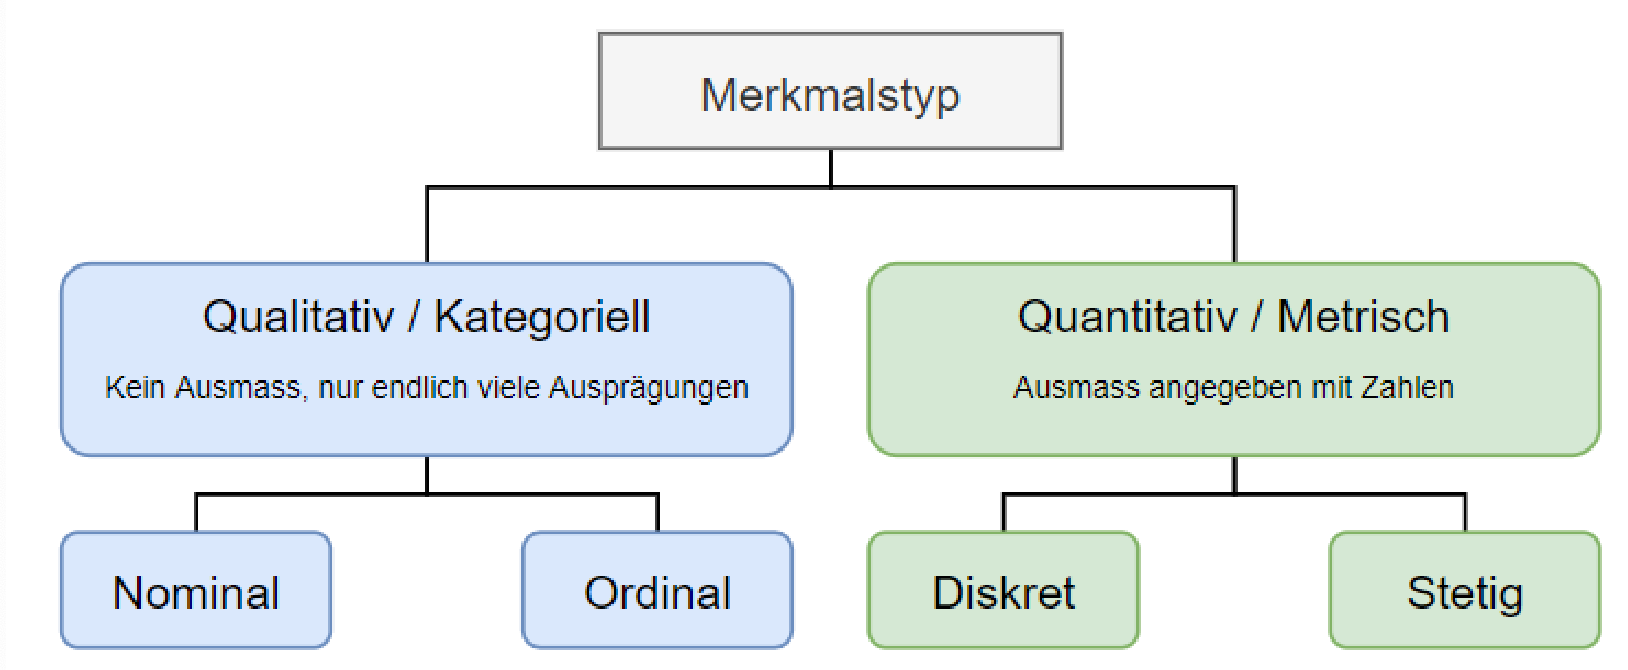
\includegraphics[width=0.8\textwidth]{images/merkmalstypen.png}
\end{center}
\end{concept}

\begin{example2}{Merkmalstypen}
    \small
\begin{itemize}
    \item \textbf{Würfelwurf (4-mal)}
    \begin{itemize}
        \item Merkmalsausprägungen: Zahlen 1 bis 6
        \item Messniveau: Metrisch diskret
    \end{itemize}
    
    \item \textbf{Parteiwahl (100 Menschen)}
    \begin{itemize}
        \item Merkmalsausprägungen: BDP, CVP, FDP, GLP, etc.
        \item Messniveau: Nominal
    \end{itemize}
    
    \item \textbf{Programmrobustheit (100 Tests)}
    \begin{itemize}
        \item Merkmalsausprägungen: schlecht, mittel, sehr gut
        \item Messniveau: Ordinal
    \end{itemize}
    
    \item \textbf{Programmlaufzeit (100 Tests)}
    \begin{itemize}
        \item Merkmalsausprägungen: Laufzeiten
        \item Messniveau: Metrisch stetig
    \end{itemize}
\end{itemize}
\end{example2}

\subsection{Häufigkeiten und Verteilungsfunktion}

\begin{concept}{Grundlegende Begriffe}
\begin{itemize}
    \item \textbf{Urliste:} Liste der beobachteten Stichprobenwerte (Messwerte)
    \item \textbf{Absolute Häufigkeit} $h_i$: Anzahl des Auftretens eines Wertes $a_i$
    \item \textbf{Relative Häufigkeit} $f_i$: Absolute Häufigkeit geteilt durch Stichprobenumfang
    \item \textbf{Empirische Dichtefunktion:} 
    \begin{itemize}
        \item Diskrete Merkmale: PMF (probability mass function)
        \item Stetige Merkmale: PDF (probability density function)
    \end{itemize}
\end{itemize}
\end{concept}

\begin{minipage}{0.5\columnwidth}
\begin{formula}{Absolute Häufigkeit H}
\vspace{-2mm}\\
    %TODO: H(X) ??
$$
H=\sum_{i=1}^{n} h_{i}
$$
\\
\small{
$h_{i}$: Einzelhäufigkeit der\\ $i$-ten Beobachtung \\
$n$: Anzahl der Beobachtungen.}
\end{formula}
\end{minipage}
\begin{minipage}{0.5\columnwidth}
\begin{formula}{Relative Häufigkeit F}
    \vspace{-2mm}\\
$$
F=\sum_{i=1}^{n} f_{i}, \quad F(x)=\frac{H(x)}{n}
$$
\small{
$f_{i}$: Einzelrelative Häufigkeit der\\ $i$-ten Beobachtung \\
$H(x)$: Absolute Häufigkeit eines\\ Wertes $x$}
\end{formula}
\end{minipage}

\begin{definition}{Absolute und Relative Häufigkeiten}
Für eine Stichprobe mit verschiedenen Merkmalsausprägungen $a_1, a_2, ..., a_m$ gilt:

\textbf{Absolute Häufigkeit:}
\begin{itemize}
    \item $h_i$ ist die Anzahl des Auftretens von $a_i$ ($i = 1,...,m$)
    \item $\sum_{i=1}^m h_i = n$ (Stichprobenumfang)
\end{itemize}

\textbf{Relative Häufigkeit:}
\begin{itemize}
    \item $f_i = \frac{h_i}{n}$ 
    \item $\sum_{i=1}^m f_i = 1$
\end{itemize}
\end{definition}

\begin{KR}{Erstellen einer Häufigkeitsverteilung}
\begin{enumerate}
    \item Sammle alle verschiedenen Werte
    \item Zähle absolute Häufigkeiten:
        \begin{itemize}
            \item Wie oft kommt jeder Wert vor?
        \end{itemize}
    \item Berechne relative Häufigkeiten:
        \begin{itemize}
            \item Teile jede absolute Häufigkeit durch $n$
        \end{itemize}
    \item Berechne kumulative Häufigkeiten:
        \begin{itemize}
            \item Absolute: Summiere $h_i$ von links nach rechts
            \item Relative: Summiere $f_i$ von links nach rechts
        \end{itemize}
\end{enumerate}
\end{KR}

\begin{example2}{Würfelwurf}
Ein Würfel wird 20 Mal geworfen:

\begin{center}
\begin{tabular}{|c|c|c|c|c|c|c|c|}
\hline
$a_i$ & 1 & 2 & 3 & 4 & 5 & 6 & Total \\
\hline 
$h_i$ & 4 & 3 & 4 & 0 & 6 & 3 & 20 \\
\hline
$f_i$ & 4/20 & 3/20 & 4/20 & 0 & 6/20 & 3/20 & 1 \\
\hline
\end{tabular}
\end{center}
\end{example2}

\begin{definition}{Kumulative Verteilungsfunktion (CDF)}
Die empirische absolute Summenhäufigkeit $H: \mathbb{R} \rightarrow \mathbb{N}_0$ ist definiert durch:
$$H(x) = \text{Anzahl aller Stichprobenwerte} \leq x \text{ bzw. } H(x) = \sum_{i:a_i\leq x} h_i$$

Die empirische relative Summenhäufigkeit $F: \mathbb{R} \rightarrow \mathbb{R}$ ist definiert durch:
$$F(x) = \frac{H(x)}{n} \text{ bzw. } F(x) = \sum_{i:a_i\leq x} f_i$$

Diese CDF ist eine Stufenfunktion, die monoton von 0 bis 1 wächst und an den Stellen $a_i$ genau um $f_i$ springt.
\end{definition}

\begin{example2}{Programmlaufzeiten}
Ein Programm wird auf 20 Rechnern ausgeführt. Folgende Laufzeiten (in ms) werden gemessen:
400, 399, 398, 400, 398, 399, 397, 400, 402, 399, 401, 399, 400, 402, 398, 400, 399, 401, 399, 399

\begin{center}
\begin{tabular}{|c|c|c|c|c|c|c|c|}
\hline
$a_i$ & 397 & 398 & 399 & 400 & 401 & 402 & Total \\
\hline
$h_i$ & 1 & 3 & 7 & 5 & 2 & 2 & 20 \\
\hline
$f_i$ & 1/20 & 3/20 & 7/20 & 5/20 & 2/20 & 2/20 & 1 \\
\hline
$H_i$ & 1 & 4 & 11 & 16 & 18 & 20 & \\
\hline
$F_i$ & 1/20 & 4/20 & 11/20 & 16/20 & 18/20 & 1 & \\
\hline
\end{tabular}
\end{center}
\end{example2}

\begin{concept}{Eigenschaften der CDF}
Für jede empirische kumulative Verteilungsfunktion $F: \mathbb{R} \rightarrow \mathbb{R}$ gilt:
\begin{itemize}
    \item $F(x) = \sum_{r\leq x} f(r)$ mit der relativen Häufigkeitsfunktion (PMF)
    \item $0 \leq F(x) \leq 1$ für alle reellen Zahlen $x$
    \item $F(x)$ ist monoton wachsend
    \item Der Graph von $F(x)$ ist eine rechtsseitig stetige Treppenfunktion
    \item Es gibt eine reelle Zahl $x$ mit $F(x) = 0$
    \item Es gibt eine reelle Zahl $y$ mit $F(y) = 1$
    \item Der Anteil aller Stichprobenwerte $x_i$ im Bereich $a < x_i \leq b$ berechnet sich als $F(b) - F(a)$
\end{itemize}
\end{concept}

\subsection{Klassierte Stichproben}

\begin{definition}{Klassierung von Daten}
Bei grossen Stichproben metrisch stetiger Merkmale teilt man die Stichprobenwerte in Klassen ein:
\begin{itemize}
    \item Die Klassen sind aneinandergrenzende Intervalle
    \item Obere Intervallgrenzen zählen immer zum darauffolgenden Intervall
    \item Relative Häufigkeit eines Intervalls = Anzahl enthaltener Stichprobenwerte / Stichprobengrösse
    \item Die relative Häufigkeit eines Intervalls entspricht der Fläche des darüber liegenden Rechtecks im Histogramm
\end{itemize}
\end{definition}

\begin{concept}{Häufigkeitsdichtefunktion}
Bei klassierten Daten wird die Häufigkeit als Rechtecksfläche über der Klassenbreite $d_i$ dargestellt:

\textbf{Absolute Häufigkeitsdichte:}
$$h = \frac{h_i}{d_i}$$

\textbf{Relative Häufigkeitsdichte:}
$$f = \frac{f_i}{d_i}$$

Die Höhe des Rechtecks entspricht der absoluten bzw. relativen Häufigkeitsdichte.
\end{concept}

\begin{example2}{Ausgaben für Transport}
Jährliche Ausgaben für Transport im ÖV von 750 Personen:

\begin{center}
\begin{tabular}{|c|c|c|c|c|c|c|}
\hline
Klasse $c_i$ & [100,200) & [200,500) & [500,800) & [800,1000) & [1000,2000) & Total \\
\hline
$h_i$ & 35 & 182 & 317 & 84 & 132 & 750 \\
\hline
$f_i$ & 35/750 & 182/750 & 317/750 & 84/750 & 132/750 & 1 \\
\hline
$d_i$ & 100 & 300 & 300 & 200 & 1000 & \\
\hline
$h(x)$ & 35/100 & 182/300 & 317/300 & 84/200 & 132/1000 & \\
\hline
$f(x)$ & 35/(750·100) & 182/(750·300) & 317/(750·300) & 84/(750·200) & 132/(750·1000) & \\
\hline
\end{tabular}
\end{center}
\end{example2}

\begin{KR}{Klassenbildung (Faustregeln)}
\begin{itemize}
    \item Die Klassen sollten gleich breit gewählt werden
    \item Die Anzahl der Klassen sollte etwa zwischen 5 und 20 liegen
    \item Die Anzahl der Klassen sollte $\sqrt{n}$ nicht wesentlich überschreiten
    \item Klassengrenzen sollten 'runde' Zahlen sein
    \item Werte auf Klassengrenzen kommen in die obere Klasse
\end{itemize}
\end{KR}

\begin{definition}{Verteilungsfunktion für klassierte Daten}
Durch Integration der relativen Häufigkeitsfunktion (PDF) $f(x)$ erhält man die kumulative Verteilungsfunktion (CDF):

$$F(x) = \int_{-\infty}^x f(t)dt$$

Dabei gilt:
\begin{itemize}
    \item $F(x)$ ist stetig und stückweise differenzierbar
    \item Die Werte von $F(x)$ an den rechten Klassengrenzen erhält man durch Kumulieren der relativen Häufigkeiten $f_i$ im kompletten Intervall
\end{itemize}
\end{definition}

\begin{KR}{Berechnung der CDF für klassierte Daten}
\begin{enumerate}
    \item Bestimme für jede Klasse:
    \begin{itemize}
        \item Klassenbreite $d_i$
        \item Absolute Häufigkeit $h_i$
        \item Relative Häufigkeit $f_i = \frac{h_i}{n}$
    \end{itemize}
    \item Kumuliere die relativen Häufigkeiten
    \item Werte der CDF:
    \begin{itemize}
        \item An linker Klassengrenze: F(x) entspricht kumulierter Häufigkeit bis vorherige Klasse
        \item An rechter Klassengrenze: F(x) entspricht kumulierter Häufigkeit bis aktuelle Klasse
        \item Dazwischen: Lineare Interpolation
    \end{itemize}
\end{enumerate}
\end{KR}

\subsection{Kenngrössen}

\begin{concept}{Arten von Kenngrössen}
Bei der Analyse von Verteilungen unterscheidet man:
\begin{itemize}
    \item \textbf{Lagemasse:} Beschreiben das Zentrum der Verteilung
    \item \textbf{Streuungsmasse:} Charakterisieren die Abweichung vom Zentrum
    \item \textbf{Schiefemasse:} Beschreiben die Form der Verteilung
\end{itemize}
\end{concept}

\subsubsection{Quantile}

\begin{definition}{Quantile}
Für eine reelle Zahl $0 \leq q \leq 1$ heisst eine Zahl $R$ ein $q$-Quantil der Stichprobe $x_1, x_2, ..., x_n$, falls:
\begin{itemize}
    \item Der Anteil der Stichprobenwerte $x_i \leq R$ mindestens $q$ ist
    \item Der Anteil der Stichprobenwerte $x_i \geq R$ mindestens $1-q$ ist
\end{itemize}

Die 0.25, 0.5 und 0.75-Quantile werden auch 1., 2. und 3. Quartil genannt.
\end{definition}

\begin{KR}{Berechnung von Quantilen}
Für eine geordnete Stichprobe $x_{[1]} \leq x_{[2]} \leq ... \leq x_{[n]}$:
\begin{enumerate}
    \item Berechne $n \cdot q$
    \item Falls $n \cdot q$ eine ganze Zahl ist:
        $$R_q = \frac{1}{2}(x_{n\cdot q} + x_{n\cdot q+1})$$
    \item Falls $n \cdot q$ keine ganze Zahl ist:
        $$R_q = x_{\lceil n\cdot q \rceil}$$
    \item Wobei $\lceil n\cdot q \rceil$ die nächstgrössere ganze Zahl ist
\end{enumerate}
\end{KR}

\begin{concept}{Median}
Das 0.5-Quantil (2. Quartil) wird auch Median oder Zentralwert genannt:
$$\text{Median}(x_1,...,x_n) = x_{\text{med}} = \begin{cases}
x_{[\frac{n+1}{2}]} & \text{falls } n \text{ ungerade}\\
\frac{1}{2}(x_{[\frac{n}{2}]} + x_{[\frac{n}{2}+1]}) & \text{falls } n \text{ gerade}
\end{cases}$$

Der Median teilt einen Datensatz in zwei gleich grosse Hälften.
\end{concept}

\subsubsection{Boxplot}

\begin{definition}{Boxplot}
Ein Boxplot besteht aus:
\begin{itemize}
    \item Box: Begrenzt durch 1. und 3. Quartil ($Q_1$ und $Q_3$)
    \item Mittellinie: Median ($Q_2$)
    \item Interquartilsabstand: $IQR = Q_3 - Q_1$
    \item Antennen (Whisker):
    \begin{itemize}
        \item Untere Antenne: Minimum der Werte $\geq Q_1 - 1.5 \cdot IQR$
        \item Obere Antenne: Maximum der Werte $\leq Q_3 + 1.5 \cdot IQR$
    \end{itemize}
    \item Ausreisser: Alle Werte ausserhalb der Antennen
\end{itemize}
\end{definition}

\begin{KR}{Erstellen eines Boxplots}
\begin{enumerate}
    \item Berechne Quartile $Q_1$, $Q_2$ (Median) und $Q_3$
    \item Bestimme Interquartilsabstand $IQR = Q_3 - Q_1$
    \item Berechne Grenzen für Ausreisser:
    \begin{itemize}
        \item Untere Grenze: $Q_1 - 1.5 \cdot IQR$
        \item Obere Grenze: $Q_3 + 1.5 \cdot IQR$
    \end{itemize}
    \item Zeichne Box und Antennen
    \item Markiere Ausreisser einzeln
\end{enumerate}
\end{KR}

\subsubsection{Lagekennwerte}

\begin{definition}{Lageparameter}
\begin{itemize}
    \item \textbf{Arithmetisches Mittel:}
    $$\bar{x} = \frac{1}{n}\sum_{i=1}^n x_i = \sum_{i=1}^m a_i \cdot f_i$$
    
    \item \textbf{Median:} Teilt Datensatz in zwei gleich grosse Hälften
    
    \item \textbf{Modus:} Häufigster Wert in der Stichprobe
\end{itemize}
\end{definition}

\subsubsection{Streuungskennwerte}

\begin{definition}{Streuungsmasse}
\textbf{Stichprobenvarianz:}
$$s^2 = \frac{1}{n}\sum_{i=1}^n (x_i - \bar{x})^2 = \frac{1}{n}\sum_{i=1}^n x_i^2 - \bar{x}^2$$

\textbf{Korrigierte Stichprobenvarianz:}
$$s_{\text{kor}}^2 = \frac{1}{n-1}\sum_{i=1}^n (x_i - \bar{x})^2 = \frac{n}{n-1}s^2$$

\textbf{Standardabweichung:}
$$s = \sqrt{s^2} \quad \text{bzw.} \quad s_{\text{kor}} = \sqrt{s_{\text{kor}}^2}$$
\end{definition}

\subsubsection{Form der Verteilung}

\begin{concept}{Verteilungsformen}
\begin{itemize}
    \item \textbf{Symmetrisch:} Rechte und linke Hälfte spiegelbildlich
    \item \textbf{Linkssteil (rechtsschief):}
    \begin{itemize}
        \item Daten links konzentriert
        \item $x_{\text{mod}} < x_{\text{med}} < \bar{x}$
    \end{itemize}
    \item \textbf{Rechtssteil (linksschief):}
    \begin{itemize}
        \item Daten rechts konzentriert
        \item $x_{\text{mod}} > x_{\text{med}} > \bar{x}$
    \end{itemize}
    \item \textbf{Modalität:}
    \begin{itemize}
        \item Unimodal: Ein Maximum
        \item Bimodal/Multimodal: Mehrere Maxima
    \end{itemize}
\end{itemize}
\end{concept}